\documentclass[dvipsnames,beamer,10pt]{standalone}

\usepackage{tikz}
\usetikzlibrary{positioning,decorations.pathreplacing,fit}
\usetikzlibrary{decorations.markings,arrows.meta,shapes.arrows,arrows}
\usetikzlibrary{calc}

\definecolor{mygreen}{RGB}{0,128,80}
\colorlet{darkgreen}{mygreen!90!black}




\begin{document}




\begin{standaloneframe}

\resizebox{0.8\textwidth}{!}{



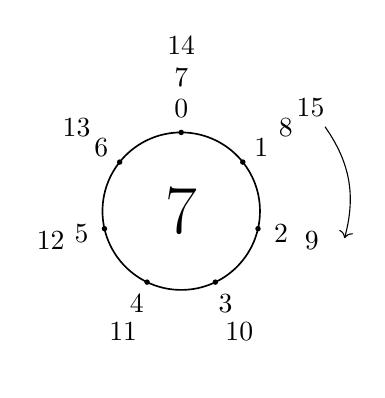
\begin{tikzpicture}[
	send/.style= {
		>={Latex[length=1pt,width=1.8pt]},shorten <= 1pt,line width=0.3pt
	},
	]
	
	
	\draw[semithick] circle(1cm) node {\Huge7};
	
	\foreach \a in {0,1,...,6}{
		\draw (-\a*360/7 + 90: 1.3cm) node{\a};
		\draw (-\a*360/7 + 90: 1cm) node [fill,circle, inner sep=0.7pt] {};
	}
	
	\uncover<2->{	
		\foreach \a in {7,...,13}{
			\draw (-\a*360/7 + 90: 1.7cm) node{\a};
		}
		\foreach \a in {14,15}{
			\draw (-\a*360/7 + 90: 2.1cm) node (p\a) {\a};
		}
		\foreach \a in {16,...,18}{
			\draw (-\a*360/7 + 90: 2.1cm) node (p\a)[] {};
		}	
		\draw[->] (p15) to [bend left=25] (p16);
	}


	

		


\end{tikzpicture}


}

\end{standaloneframe}


\end{document}